\documentclass{article}
\usepackage[utf8]{inputenc}
\usepackage{graphicx}
\title{\LaTeX{} and Gnuplot: the Gamma function}
\author{Esben Hygum Larsen}
\date{\today}

\begin{document}
\maketitle
The gamma function is defined as:
\begin{equation}
    \Gamma (n)=(n-1)!\ .
\end{equation}
\noindent where n is a positive integer. It can also be defined for a complex number with a positive real part:

\begin{equation}
    \Gamma (z)=\int _{0}^{\infty }x^{z-1}e^{-x} dx, \qquad \Re (z)>0
\end{equation}


\begin{figure}
    \centering
    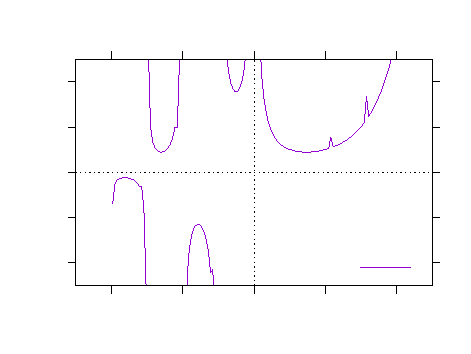
\includegraphics[width = 0.95\columnwidth]{plot-gamma-eps-converted-to.pdf}
    \caption{Gamma function}
\end{figure}

\end{document}
